\documentclass[12pt,a4paper]{article}
\usepackage[utf8]{inputenc}
\usepackage[spanish]{babel}
\usepackage{amsmath}
\usepackage{amsfonts}
\usepackage{amssymb}
\usepackage{graphicx}
\usepackage[left=2cm,right=2cm,top=2cm,bottom=2cm]{geometry}
\author{Enciso Guerrero Benjamin Salvador\\
Carlos Enrrique Moran Garabito\\
Cinematica De Robots }
\title{Convención denavit-hartenberg.}
\begin{document}
\maketitle

\includegraphics[scale=1.8]{upzmgg.jpg} 
\newpage
\textbf{CONVENCION DENAVIT-HARTENBERG.}
\\\\
Se trata de un procedimiento sistemático para describir la estructura cinemática de una cadena articulada constituida por articulaciones con. un solo grado de libertad. Para ello, a cada articulación se le asigna un Sistema de Referencia Local con origen en un punto Qi y ejes ortonormales {Xi, Yi, Zi}, comenzando con un primer S.R fijo e inmóvil dado por los ejes {X0, Y0, Z0}, anclado a un punto fijo Q0 de la Base sobre la que está montada toda la estructura de la cadena. Este Sistema de Referencia no tiene por qué ser el Universal con origen en (0,0,0) y la Base canónica.\\\\
\textbf{ASIGNACIÓN DE EJES}
\\\\
1-Enumerar los n+1 eslabones de 0 a n, comenzando desde la base (eslabón fijo) y terminando en el efector final.
\\\\
2-Identificar los ejes de cada articulación. Si es rotacional será el eje de giro, y si es prismática será el eje a lo largo del cual se produce el desplazamiento.
\\\\
3-Enumerar los ejes de 1 a n comenzando desde el que une eslabón base con el eslabón 1.
\\\\
4-Para de 0 a n-1: situar el eje Zi en el eje de articulación i+1
\\\\
5-El eje Zn se colocará en el extremo del último eslabón, en la misma dirección que el Zn-1.
\\\\
6-Situar el origen del sistema de la base {S0} en cualquier punto del eje Z0.
\\\\
7-Para i de 1 a n: situar el sistema {Si} en la intersección entre el eje Zi y la recta que es perpendicular simultáneamente al eje Zi y al eje Zi-1. Si los ejes Zi y Zi-1 se cortan el sistema {Si} se coloca en el punto de intersección
\\\\
8-Para i de 1 a n: situar el eje Xi a partir del punto donde se definió el {Si} sobre la recta que es perpendicular simultáneamente al eje Zi y al eje Zi-1. Si los ejes Zi y Zi-1 se cortan el eje Xi debe ser perpendicular a ambos. El sentido es indiferente.
\\\\
9-El X0 se puede colocar libremente. Puede resultar útil que esté alineado con el X1.
\\\\
10-Para i de 0 a n: colocar el eje Yi de modo que forme un sistema dextrógiro con los ejes Xi y Zi.
\\\\
\textbf{DETERMINACIÓN DE PARÁMETROS}
\\\\
Para i de 0 a n:
\\\\
1-0i: Ángulo alrededor del eje Zi-1, desde el eje Xi-1 hasta el eje Xi-.
\\\\
2-Di: Distancia a lo largo del eje Zi-1, desde el origen del sistema i-1 hasta el eje Xi.
\\\\
3-Ai: Distancia a lo largo del eje Xi, desde el eje Zi-1 hasta el eje Zi-.
\\\\
4.B: Ángulo alrededor del eje Xi, desde el eje Zi-1 hasta el eje Zi-.
\\
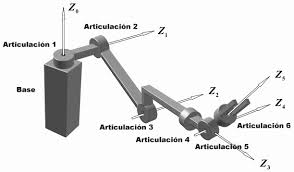
\includegraphics[scale=1.5]{grados.jpg} \\
Figura con definición de las articulaciones.
\\\\
La representación Denavit-Hartenberg presupone que cuando se realiza una rotación alrededor de uno de los ejes, digamos Zi- 1, la orientación del eje Zi varía debido a la acción del brazo que los une (exceptuando el caso en el que Zi- 1 y Zi son paralelos), aunque naturalmente el ángulo i(alfa) entre ambos ejes permanece constante. 
\\\\
Esta observación implica que es imposible que el eje Zi tenga una orientación constante e independiente de la rotación que se efectúe alrededor de Zi- 1, lo cual implica que la transformación de un sistema a otro no puede en ningún caso expresarse como una rotación de ángulos de Euler de Ejes Fijos, como la RPY.




\end{document}